The SMs are the computational working blocks of the GPU.
It handles all tasks submitted to the GPU, which is executed in its sub blocks.
\Cref{fig:hw-sm} presents the hardware architecture of a basic SM, containing:

\begin{itemize}
	\item Instruction Buffer
	\item One or more Warp Scheduler(s)
	\item Warp Scheduler
	\item Streaming Processor
	\item Special Function Units
	\item Register File
	\item L1 Cache
	\item Shared Memory
\end{itemize}

%SFU
Special Function Units (SFUs) are a approximation units, which computes fast single-precision approximations of transcendental functions such as logarithm, exponential, sine and cosine \cite{Wilt2013}.
Each of the SFUs also contains four floating-point multipliers that can offer extra throughput in addition to the SPs\cite{Li2016}.

\begin{figure}[H]
	\centering
	\fbox{
		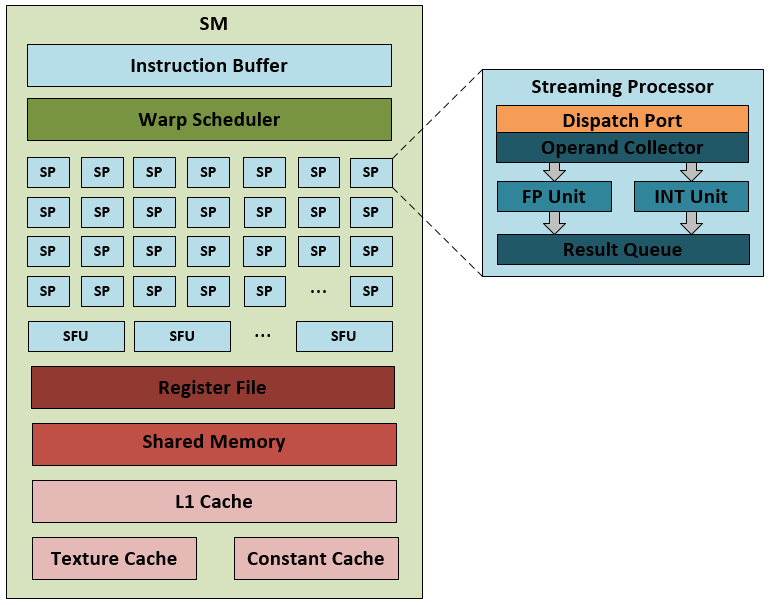
\includegraphics[width=1\textwidth]{figs/hw/hw-sm} }
	\caption{TBD}
	\label{fig:hw-sm}
\end{figure}